% Softening Duffing oscillator as the roll motion of a ship: roll angle phi
% between the vertical and the ship's axis, input torque u at the keel.
% Ship geometry and colours as in ship_rolling_simulation.py.
\documentclass[tikz, border=4pt]{standalone}
\usetikzlibrary{arrows.meta}

\definecolor{water}{HTML}{A8D0E6}
\definecolor{waterline}{HTML}{3A7CA5}
\definecolor{hull}{HTML}{5A7A3F}

\begin{document}
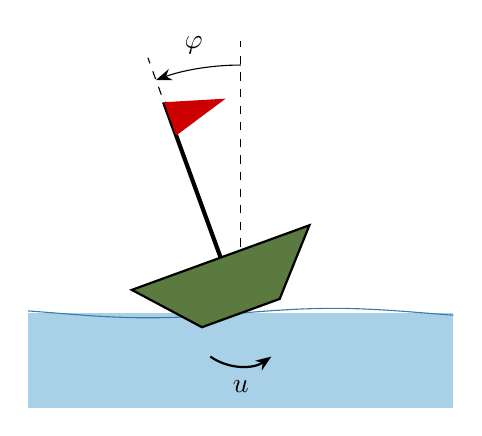
\begin{tikzpicture}[>={Stealth[length=2mm]}, scale=1.5]
  \def\phiShip{20}  % displayed roll angle [deg], counter-clockwise positive

  % water
  \fill[water] (-1.8, -0.8) rectangle (1.8, 0);
  \draw[waterline, domain=-1.8:1.8, samples=60]
    plot (\x, {0.04*sin(115*\x)});

  % vertical reference and the ship's axis
  \draw[dashed] (0, 0) -- (0, 2.3);
  \draw[dashed] (0, 0) -- (90+\phiShip:2.3);

  % ship, rolled about the bottom of the hull
  \begin{scope}[rotate=\phiShip]
    \filldraw[fill=hull, draw=black, thick]
      (-0.35, 0) -- (0.35, 0) -- (0.8, 0.5) -- (-0.8, 0.5) -- cycle;
    \draw[line width=1.5pt] (0, 0.5) -- (0, 1.9);
    \fill[red!80!black] (0, 1.9) -- (0.5, 1.75) -- (0, 1.6) -- cycle;
  \end{scope}

  % roll angle
  \draw[->] (90:2.1) arc[start angle=90, end angle=90+\phiShip, radius=2.1];
  \node at (90+\phiShip/2:2.3) {$\varphi$};

  % input torque at the bottom of the ship
  \draw[->, thick] (235:0.45) arc[start angle=235, end angle=305, radius=0.45];
  \node at (270:0.62) {$u$};
\end{tikzpicture}
\end{document}
